%!TEX root = ../thesis.tex

\section{経路追従}
経路追従(Path following)とは, 経路計画(Path planning)で引いた経路に対して安全にロボットが経路を追従できるようにロボットを制御することである.
基本的にはロボットのモデルと制御アルゴリズムを利用することで, 最終的にロボットの入力値(ステアリング角度や並進速度)を計算することが目的となる.

\subsection{PurePursuit}
PurePursuitアルゴリズムは, 経路追従アルゴリズムの中で最も基礎的だが, 非常に広く使われているアルゴリズムである.

PurePursuitはFig.3.1に示すように目標経路上(Path)に対して一定距離先の点を目標点(Look Ahead)とし, その点に到達するようなステアリング制御を行う.
目標点に対してロボットが前進することで, より先の目標点にたどり着くように制御を行うため, 結果的に目標経路に追従する形となる.

\begin{figure}[H]
  \centering
 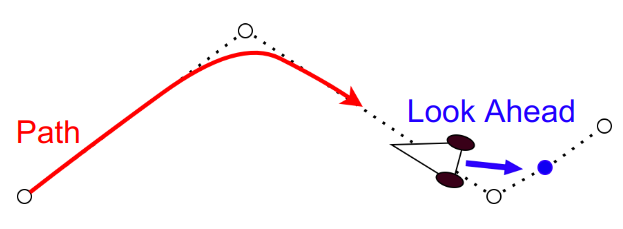
\includegraphics[keepaspectratio, scale=0.5]
      {images/PurePursuit.png}
 \caption{PurePursuit Algorithm}
 \label{fig:purepursuit}
\end{figure}

\subsection{PID制御}
PID制御(Proportional-Integral-Differential Controller)は, 制御工学におけるフィードバック制御の一種である.
出力値と目標値との偏差, その積分, および微分の3つの要素によって, 入力値の制御を行う方法である.

\subsubsection{P制御}
基本的なフィードバック制御として比例制御(P制御)がある.
これは操作量を制御量と目標値の偏差の一次関数として制御するものである.
PID制御では, この偏差に比例して操作量を変化させる動作を比例動作, またはP動作といい, その時の定数は比例ゲイン, Pゲインと呼ばれる.

\subsubsection{I制御}
P制御において, 周囲の環境が変わるたびに残留偏差をなくすように比例ゲインを決定しなおすことが難しい.
そこで, 残留偏差が存在する場合, その偏差の時間積分に比例して入力値を変化させる動作をする項を追加する.
追加した項が持つ役割がI制御である.
偏差のある状態が長い時間続けばそれだけ入力値の変化を大きくして目標値に近づけようとする役目を果たす.
ここで, 定数は積分ゲイン, Iゲインと呼ばれる.

\subsubsection{D制御}
PI制御の問題点として, 周囲の環境が変化したり制御対象に撹乱が加わったりすることで出力値が急に変動することがある.
この問題を解決するために, 急激な出力値の変化が起こった場合, その変化の大きさに比例した入力を行うことでその変化に抵抗する役割を持つ項を追加する.
追加した項が持つ役割がD制御である.
定数は微分ゲイン, Dゲインと呼ばれる.

\section{経路生成}
経路追従を行うためには, 追従するための目標経路(Path)を設定する必要がある.
自律移動ロボットの開発に置いて目標経路の探索を経路計画と呼び, 重要な問題の一つとされている.
本研究では, 目標経路は予め取得した測地座標系の経緯度で用意されたウェイポイントをつなぐライン上で定めている.


\subsection{スプライン補間}
本研究で取得する目標経路は, ウェイポイントを繋ぐライン上で定めている.
定めたウェイポイントが疎らである場合に, ロボットに無理のない追従を行わせるためには目標経路の曲線が滑らかである必要がある.
そこで, 3次スプライン補間を行うことで, 用意されたウェイポイント上を繋ぐラインに対して曲線を担保することが可能となる.

3次スプライン補間とは, 複数のサンプル点が与えられた時に, そのサンプル点の間を3次の多項式で近似し, 滑らかに保管する手法である.
Fig.3.2にその様子を示す.

\begin{figure}[H]
     \centering
    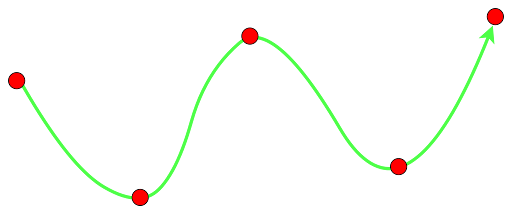
\includegraphics[keepaspectratio, scale=0.5]
         {images/splinepath.png}
    \caption{Spline path}
    \label{fig:purepursuit}
\end{figure}


\newpage